% CE6190 Group Project 2 -- report built from the A100 receiver run (2026-11-10/13).
% Every number comes from files under /home/ecs-user/ce6190-runtime/a100x8-20261110 (see Reproducibility).
% Sections marked \pending are filled only after the frozen test (Phase C) and VBench have completed.
\documentclass[11pt,a4paper]{article}
\usepackage[margin=24mm]{geometry}
\usepackage[T1]{fontenc}
\usepackage{lmodern}
\usepackage{microtype}
\usepackage{amsmath,amssymb}
\usepackage{booktabs,tabularx,array,longtable}
\usepackage{graphicx}
\usepackage{xcolor}
\usepackage{enumitem}
\usepackage{fancyhdr}
\usepackage{natbib}
\usepackage[hidelinks]{hyperref}
\usepackage{url}
\definecolor{draftorange}{RGB}{143,68,0}
\newcommand{\pending}{\textcolor{draftorange}{\textsf{TBD}}}
\newcommand{\fillin}[1]{\textcolor{draftorange}{[\textsf{Fill: #1}]}}
\newcolumntype{Y}{>{\raggedright\arraybackslash}X}
\setlength{\parindent}{0pt}
\setlength{\parskip}{5pt}
\setlength{\headheight}{15pt}
\setlist{nosep,leftmargin=*}
\pagestyle{fancy}
\fancyhf{}
\fancyhead[L]{\small CE6190 Group Project 2}
\fancyhead[R]{\small\textcolor{draftorange}{DRAFT: frozen-test results pending}}
\fancyfoot[C]{\thepage}
\title{Efficient Text-to-Video Generation via Adaptive Caching\\
\large A Controlled Comparison of TeaCache, MagCache, SeaCache and SenCache on Wan2.1-T2V-1.3B}
\author{Group \fillin{XX}\\\fillin{member names and student identifiers}}
\date{CE6190, November 2026}

\begin{document}
\maketitle
\thispagestyle{fancy}

\begin{abstract}\sloppy
We compare four training-free residual-caching policies for text-to-video diffusion---TeaCache, MagCache, SeaCache and
SenCache---against uncached inference on a single pinned Wan2.1-T2V-1.3B checkpoint (81 frames, $832\times480$, 50 UniPC
steps, CFG 5), with unmodified official decision code, one shared generation loop and per-run provenance checks. On a
validation grid of 1{,}411 generations on A100-SXM4-80GB GPUs we measure the full speed--fidelity trade-off. The FP32 VAE
decode costs $\approx$98.5\,s of the 271.4\,s uncached run, which caps end-to-end speedup at $\approx$1.72$\times$ on this
GPU; we therefore freeze thresholds at a 2.0$\times$ \emph{denoising-loop} budget. At matched denoising speedup
($2.37\times$) MagCache stays far closer to the uncached output than TeaCache (LPIPS 0.074 vs.\ 0.127), and SeaCache
attains the lowest error of all policies at moderate budgets (LPIPS 0.044 at $2.06\times$). Ablations show that
SeaCache's spectral filter is essential (an unfiltered proxy reuses aggressively and raises LPIPS to $\approx$0.6), and that
SenCache's decisions are driven by its time term. Trace analysis reveals that, on Wan, only SeaCache produces materially
prompt-dependent refresh schedules. \pending{} [held-out VBench-prompt test with frozen thresholds: fidelity and VBench
dimensions to be inserted].
\end{abstract}

\section{Introduction}
Video diffusion transformers repeatedly evaluate a large network while updating a video latent. Caching reduces this cost by
reusing the residual of the transformer block stack at denoising steps where the network output is predicted to change
little. The central decision is \emph{when} a stale residual is still an adequate approximation. TeaCache~\citep{liu2025teacache}
and MagCache~\citep{ma2025magcache} use cheap timestep-embedding or calibrated magnitude signals; SeaCache~\citep{chung2026seacache}
measures change in a spectrally filtered input representation; SenCache~\citep{haghighi2026sencache} combines latent and
timestep drift weighted by calibrated sensitivities.

We answer three questions with our own measurements:
\begin{enumerate}[label=RQ\arabic*.]
\item At matched measured speedup, how far does each policy's video deviate from the uncached video (PSNR/SSIM/LPIPS), and
\pending{} how do VBench quality dimensions compare on held-out prompts?
\item Which decision components explain SeaCache's and SenCache's behaviour (controlled ablations)?
\item Are the refresh schedules actually sample-dependent, and where in the trajectory do policies refresh?
\end{enumerate}
Our contributions are a controlled, provenance-checked benchmark (identical checkpoint, sampler, attention backend and
generation loop for every policy), a measurement of how a hardware-dependent fixed cost (the VAE decode) changes the
achievable budget, and trace-level evidence about adaptivity.

\section{Background and Methods}
\subsection{Generation and residual caching}
Wan~\citep{wan2025wan} is a flow-matching video diffusion transformer. With latent $z_t$, text condition $c$ and frozen
parameters $\theta$, each sampling step evaluates $p_t=v_\theta(z_t,t,c)$ and updates $z_s=\operatorname{Update}(z_t,p_t,t,s)$
with the UniPC solver. Classifier-free guidance (CFG) evaluates a conditional and an unconditional branch per step, i.e.\
100 transformer calls for 50 steps. For the block stack with input $h_k^{\mathrm{in}}$ and output $h_k^{\mathrm{out}}$ at call
$k$, all four policies cache the residual
\begin{equation}
r_k=h_k^{\mathrm{out}}-h_k^{\mathrm{in}},\qquad \widetilde h_k^{\mathrm{out}}=h_k^{\mathrm{in}}+r_j\quad(j<k\text{ the last refresh}),
\end{equation}
so the latent keeps updating at every step while the block computation is skipped. Our harness verifies this shared
residual contract by AST-comparing each official forward against the Wan forward before any run.

\subsection{Compared policies (as audited in the code that ran)}
All four official forwards were loaded unchanged from pinned commits (Table~\ref{tab:protocol}); the harness only sets
their documented attributes. Each CFG branch keeps its own cached residual, and in all our traces the two branches took
identical refresh decisions (0 disagreements in 4{,}300 steps per policy).
\begin{itemize}
\item \textbf{TeaCache} accumulates a polynomially rescaled relative-L1 change of the timestep-modulation input and refreshes
when the sum exceeds the threshold. With the official Wan default (\texttt{use\_ret\_steps}=False) this input is the
timestep embedding, so the decision is a function of the timestep only. First and last calls are protected.
\item \textbf{MagCache} accumulates an error predicted from a calibrated table of 100 residual-magnitude ratios (reused
handoff profile), refreshes when it exceeds the threshold, allows at most $K=4$ consecutive reuses, and protects the first
20\% of calls (retention ratio 0.2).
\item \textbf{SeaCache} uses the same accumulate-and-refresh rule as TeaCache but measures the relative change of the
input features after a timestep-aligned spectral (SEA) filter with gain normalisation (\texttt{norm\_mode=mean}); it is the
only policy whose score depends on the content of the current latent.
\item \textbf{SenCache} scores $E=s_x(t_r)\lVert z_t-z_{t_r}\rVert_2+s_t(t_r)|t-t_r|$ with calibrated per-timestep
sensitivities (reused handoff profile, timestep grid checked against the scheduler), uses a stricter start threshold
(0.045) for the first 20\% of steps, and allows at most $K=3$ consecutive reuses.
\end{itemize}

\section{Experimental Protocol}
\subsection{Data separation and shared settings}
Thresholds were selected on 33 development prompts (validation grid); calibration prompts and development prompts are
disjoint from the held-out test prompts, which we draw from VBench~\citep{huang2024vbench}. The manifest builder's
overlap check was run against both sets before generating the test manifest.

\begin{table}[htbp]
\centering\small
\begin{tabularx}{\linewidth}{@{}p{0.27\linewidth}Y@{}}\toprule
Field & Setting used\\\midrule
Checkpoint & Wan2.1-T2V-1.3B; content fingerprint \texttt{b6725fb6\ldots{}4eba4}, verified per file (size + SHA-256)\\
Code revisions & Wan \texttt{9737cba}, TeaCache \texttt{7c10efc}, MagCache \texttt{df81cb1}, SeaCache \texttt{8dcf490},
SenCache \texttt{3fb96a4}; official forwards unmodified; commit and code hashes recorded per run\\
Validation prompts & 33 development prompts, seeds 0--2, 15 policies (uncached + 14 cached) $\Rightarrow$ 97 prompt--seed
pairs; this receiver run executed 1{,}411 cells on A100 (the remaining cells had been run on H200 by the sender and are
excluded, since timings may not be mixed across hardware)\\
Test prompts & 110 VBench prompts (10 per dimension $\times$ 16 dimensions, deterministic hash order, disjoint from
development/calibration); seeds 0--4, and 25 seeds for temporal-flickering prompts; 3{,}750 runs\\
Video & 81 frames, $832\times480$, 16 fps; frames saved as uint8 arrays (metrics) and MP4 (viewing)\\
Sampling & UniPC, 50 steps, flow shift 5, CFG 5, Wan's default negative prompt, same initial noise per seed for all
policies\\
Numerics & BF16 transformer, FlashAttention-2, no offload, no compilation; FP32 VAE; TF32 off\\
Hardware/software & 8$\times$ A100-SXM4-80GB (driver 580.126.09), one process per GPU; PyTorch 2.6.0+cu124, cuDNN 9.1.0,
flash-attn 2.7.4.post1, diffusers 0.32.2, transformers 4.49.0\\
Calibration & MagCache ratios and SenCache sensitivities reused from the handoff (same fingerprint and revisions);
TeaCache uses the published 1.3B coefficients; SeaCache needs none\\
Selection & thresholds TeaCache \{0.04,0.08,0.12,0.16\}, MagCache \{0.06,0.12,0.24\}, SeaCache \{0.1,0.2,0.35\},
SenCache \{0.5,1,2,4\}; rule: lowest LPIPS among settings reaching the budget\\
Run accounting & validation 1{,}411/1{,}411 complete, 0 failed, 0 retries; all passed acceptance (status, 100 calls
$\times$ 3 traces, uncached never reuses, frame shape/dtype, MP4 decodes, fingerprint, revisions, cuDNN, dependency lock);
ablations 336/336; test \pending\\\bottomrule
\end{tabularx}
\caption{Shared settings. All policies run through the same Wan generation loop; only the cache decision differs.}
\label{tab:protocol}
\end{table}

\subsection{Metrics and timing}
\textbf{Agreement} with the uncached video of the same prompt and seed is measured on all 81 decoded uint8 frames before
video compression: PSNR (data range 255, from the pooled MSE), SSIM and LPIPS (AlexNet, v0.1). The uncached output is a
reference, not ground truth. \textbf{Quality} on held-out prompts is measured with VBench (pinned commit \texttt{fd18b3d})
on our custom subset; we do not report it as a full-benchmark score. \pending{}

\textbf{Timing} is GPU-synchronised wall time of text encoding + denoising + VAE decoding, excluding model loading and file
I/O. On the validation grid each run used one warm-up and three timed repeats in a fresh process (the reported time is
their mean; across all 1{,}411 runs the spread of the three repeats had median 0.08\,s and maximum 0.5\,s, at most 0.27\%
of the run time, and the repeats always produced identical refresh schedules). Speedup is the ratio of
summed paired times, $\sum T_{\text{uncached}}/\sum T_m$, reported end-to-end and for the denoising loop alone. Uncertainty
uses a prompt-cluster bootstrap (2{,}000 draws), so seeds of one prompt are never treated as independent samples.

\subsection{Matched budget}
The pre-registered rule froze thresholds at a measured 2.0$\times$ end-to-end speedup. On A100 this budget is unreachable:
the FP32 VAE decode takes 98.5\,s regardless of policy (Table~\ref{tab:efficiency}) and the fastest settings reach only
1.65--1.72$\times$; the official selection routine reports ``MagCache cannot reach 2.0$\times$''. Because caching only
accelerates the denoising loop, we freeze at a \textbf{2.0$\times$ denoising-only} budget with the same rule (lowest LPIPS
among settings that reach it). This keeps the intended compute budget on the accelerated part and comparability with the
sender's H200 run, where the VAE decode is $\approx$9\,s. The selected thresholds are TeaCache 0.12, MagCache 0.12, SeaCache
0.2 and SenCache 0.5 ($\star$ in Table~\ref{tab:grid}).

\section{Results and Analysis}
\subsection{Speed--fidelity trade-off on the validation grid}
\begin{table}[htbp]\centering\small\setlength{\tabcolsep}{4pt}
\begin{tabular}{@{}llrrrcrrl@{}}\toprule
Method & Thr. & Total (s) & Denoise (s) & VAE (s) & Speedup E2E / Den. & Full calls & Peak GB & Calib.\\\midrule
Uncached & -- & 271.4 & 172.7 & 98.5 & 1.00 / 1.00 & 100 & 25.9 & n/a \\
TeaCache & 0.12 & 171.6 & 72.9 & 98.6 & 1.58 / 2.37 & 42 & 26.2 & none \\
MagCache & 0.12 & 171.5 & 72.9 & 98.5 & 1.58 / 2.37 & 42 & 26.2 & reused \\
SeaCache & 0.2 & 182.4 & 83.6 & 98.6 & 1.49 / 2.06 & 48 & 26.6 & none \\
SenCache & 0.5 & 164.9 & 66.2 & 98.6 & 1.65 / 2.61 & 38 & 25.9 & reused \\
\bottomrule\end{tabular}
\caption{Latency at the frozen settings on the validation grid (86 pairs; per-run time is the mean of 3 timed repeats after
one warm-up, GPU-synchronised, model loading excluded). Full calls: full block-stack evaluations per video out of 100
(50 UniPC steps $\times$ 2 CFG branches). The FP32 VAE decode ($\approx$98.5\,s, identical for all methods) bounds the
end-to-end speedup on this GPU. Calibration: MagCache ratios and SenCache sensitivity profiles were reused from the
handoff package (same checkpoint fingerprint); their one-off calibration time was not re-measured here.}
\label{tab:efficiency}\end{table}

\begin{table}[htbp]\centering\small
\begin{tabular}{@{}llrrrrrl@{}}\toprule
Method & Thr. & E2E $\times$ & Denoise $\times$ & Refresh & PSNR$\uparrow$ & SSIM$\uparrow$ & LPIPS$\downarrow$ [95\% CI]\\\midrule
TeaCache & 0.04 & 1.23 & 1.43 & 0.70 & 32.08 & 0.948 & 0.030 [0.024, 0.036] \\
 & 0.08 & 1.46 & 1.99 & 0.50 & 24.08 & 0.837 & 0.112 [0.098, 0.126] \\
 & 0.12$^\star$ & 1.58 & 2.37 & 0.42 & 23.51 & 0.820 & 0.127 [0.112, 0.140] \\
 & 0.16 & 1.72 & 2.92 & 0.34 & 21.73 & 0.777 & 0.171 [0.155, 0.187] \\
\addlinespace
MagCache & 0.06 & 1.44 & 1.92 & 0.52 & 27.54 & 0.900 & 0.063 [0.054, 0.072] \\
 & 0.12$^\star$ & 1.58 & 2.37 & 0.42 & 27.11 & 0.890 & 0.074 [0.063, 0.083] \\
 & 0.24 & 1.65 & 2.62 & 0.38 & 26.91 & 0.884 & 0.079 [0.068, 0.090] \\
\addlinespace
SeaCache & 0.1 & 1.23 & 1.42 & 0.70 & 38.94 & 0.983 & 0.010 [0.008, 0.014] \\
 & 0.2$^\star$ & 1.49 & 2.06 & 0.48 & 30.88 & 0.936 & 0.044 [0.036, 0.052] \\
 & 0.35 & 1.71 & 2.88 & 0.34 & 24.92 & 0.837 & 0.117 [0.102, 0.130] \\
\addlinespace
SenCache & 0.5$^\star$ & 1.65 & 2.61 & 0.38 & 23.73 & 0.828 & 0.123 [0.109, 0.136] \\
 & 1 & 1.71 & 2.87 & 0.35 & 23.65 & 0.822 & 0.129 [0.114, 0.143] \\
 & 2 & 1.72 & 2.92 & 0.34 & 23.63 & 0.821 & 0.130 [0.115, 0.144] \\
 & 4 & 1.72 & 2.92 & 0.34 & 23.63 & 0.821 & 0.130 [0.115, 0.144] \\
\bottomrule\end{tabular}
\caption{Validation (tune) grid on A100-SXM4-80GB: 86 prompt--seed pairs common to all policies (29 development prompts
$\times$ seeds 0--2). Speedups are ratios of summed times against the paired uncached runs (E2E includes text encoding,
denoising and VAE decoding; ``Denoise'' is the denoising loop only). Refresh is the fraction of the 100 CFG-branch calls
that ran the full block stack. Agreement metrics compare against the same-seed uncached frames; means over prompts with
prompt-cluster bootstrap CIs (2000 draws). $^\star$: frozen setting (2.0$\times$ denoising-only budget).}
\label{tab:grid}\end{table}

\begin{figure}[htbp]\centering
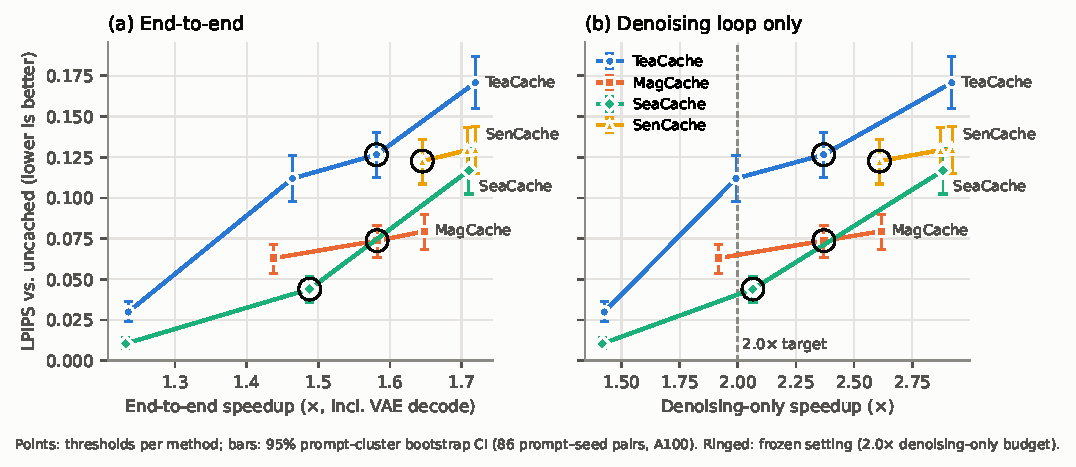
\includegraphics[width=\linewidth]{figures/pareto_speed_lpips.pdf}
\caption{Speed--fidelity trade-off on the validation grid (86 pairs). Left: end-to-end speedup; right: denoising-loop
speedup. Error bars: 95\% prompt-cluster bootstrap CIs. Rings mark the frozen settings.}
\label{fig:pareto}
\end{figure}

Table~\ref{tab:efficiency} shows where time goes: denoising accounts for 172.7\,s and the VAE decode for 98.5\,s of the
271.4\,s uncached run; caching changes only the former and leaves peak memory almost unchanged (25.9--26.6\,GB).
Figure~\ref{fig:pareto} and Table~\ref{tab:grid} give the full trade-off. Three observations hold with non-overlapping
confidence intervals:
\begin{itemize}
\item \textbf{MagCache vs.\ TeaCache at identical cost.} At the frozen settings both perform 42 of 100 full calls and reach
1.58$\times$ (2.37$\times$ denoising), yet MagCache's LPIPS is 0.074 [0.063, 0.083] against 0.127 [0.112, 0.140] and its
PSNR is 3.6\,dB higher. The calibrated magnitude table places refreshes where the residual actually changes.
\item \textbf{SeaCache is best at low and moderate budgets.} At 1.23$\times$ it is nearly lossless (LPIPS 0.011, PSNR
38.9\,dB) and at 1.49$\times$ it attains LPIPS 0.044, the lowest of any policy above 2$\times$ denoising speedup. All three
SeaCache settings lie on the latency--LPIPS Pareto front.
\item \textbf{At the highest budgets the policies converge.} Near 1.71$\times$ (34 full calls) SeaCache (0.117),
SenCache (0.129--0.130) and TeaCache (0.171) all degrade; SenCache saturates at refresh 0.34 for thresholds $\geq1$ because
its skip limit ($K=3$) and protected steps bound how much can be skipped.
\end{itemize}

\subsection{Where the policies refresh}
\begin{figure}[htbp]\centering
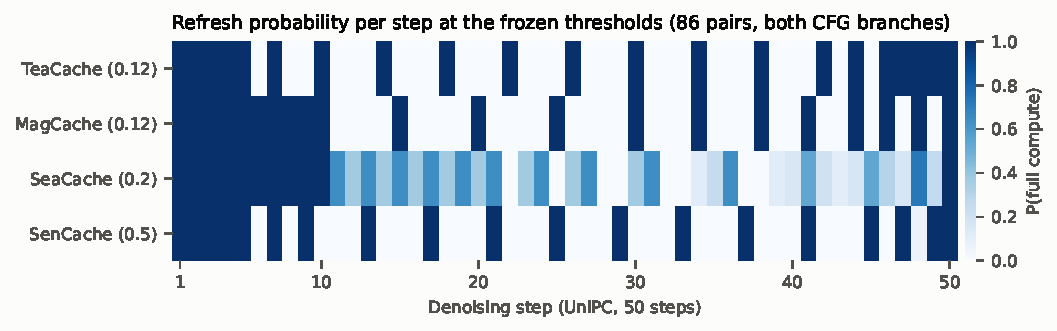
\includegraphics[width=\linewidth]{figures/refresh_schedule.pdf}
\caption{Probability of a full block-stack evaluation at each denoising step, at the frozen thresholds (86 pairs).}
\label{fig:schedule}
\end{figure}
Figure~\ref{fig:schedule} shows that all policies compute the early, high-noise steps in full (TeaCache and SenCache the
first 5, MagCache and SeaCache the first 10--11) and refresh again near the end. Across the 86 validation pairs TeaCache and
MagCache produced a \emph{single} schedule, SenCache two and SeaCache nine distinct schedules. TeaCache's Wan proxy depends
only on the timestep and MagCache's on a fixed calibration table, so their ``adaptive'' decisions are in fact static
schedules for a given sampler; SenCache's latent term rarely changes a decision at this threshold (see ablations). Only
SeaCache adapts to content: after its protected start, 30 of 38 steps have a refresh probability strictly between 0.05
and 0.95 (range 0--0.72). This answers RQ3:
on this backbone, sample dependence is a property of SeaCache's spectral proxy rather than of caching in general.

\subsection{Component ablations}
\begin{table}[htbp]\centering\small
\begin{tabular}{@{}llrrrrrr@{}}\toprule
Variant & Thr. & Pairs & Refresh & E2E $\times$ & PSNR & SSIM & LPIPS\\\midrule
SeaCache official & 0.1 & 21 & 0.70 & 1.23 & 37.73 & 0.970 & 0.015 \\
 & 0.2 & 21 & 0.48 & 1.49 & 29.8 & 0.917 & 0.053 \\
 & 0.35 & 21 & 0.34 & 1.71 & 24.3 & 0.787 & 0.136 \\
\addlinespace
SeaCache no gain normalisation & 0.1 & 21 & 1.00 & 1.00 & $\infty$ & 1.000 & 0.000 \\
 & 0.2 & 21 & 0.74 & 1.19 & 36.69 & 0.967 & 0.017 \\
 & 0.35 & 21 & 0.53 & 1.43 & 28.48 & 0.897 & 0.058 \\
\addlinespace
SeaCache raw (unfiltered) proxy & 0.1 & 21 & 0.25 & 1.91 & 14.34 & 0.474 & 0.601 \\
 & 0.2 & 21 & 0.15 & 2.18 & 14.13 & 0.469 & 0.639 \\
 & 0.35 & 21 & 0.10 & 2.34 & 14.05 & 0.464 & 0.662 \\
\addlinespace
SenCache official & 0.5 & 24 & 0.38 & 1.65 & 23.25 & 0.787 & 0.139 \\
 & 1 & 24 & 0.34 & 1.71 & 23.2 & 0.781 & 0.145 \\
 & 2 & 24 & 0.34 & 1.72 & 23.19 & 0.781 & 0.146 \\
 & 4 & 24 & 0.34 & 1.72 & 23.19 & 0.781 & 0.146 \\
\addlinespace
SenCache time term only & 0.5 & 24 & 0.34 & 1.72 & 23.19 & 0.781 & 0.146 \\
 & 1 & 24 & 0.34 & 1.72 & 23.19 & 0.781 & 0.146 \\
 & 2 & 24 & 0.34 & 1.72 & 23.19 & 0.781 & 0.146 \\
 & 4 & 24 & 0.34 & 1.72 & 23.19 & 0.781 & 0.146 \\
\addlinespace
SenCache latent term only & 0.5 & 24 & 0.29 & 1.81 & 16.1 & 0.540 & 0.412 \\
 & 1 & 24 & 0.28 & 1.84 & 16.14 & 0.541 & 0.416 \\
 & 2 & 24 & 0.28 & 1.84 & 16.14 & 0.541 & 0.416 \\
 & 4 & 24 & 0.28 & 1.84 & 16.14 & 0.541 & 0.416 \\
\bottomrule\end{tabular}
\caption{Component ablations on the validation prompts (A100). Each variant is compared with the official policy on the
same prompt--seed pairs whose official runs were measured on this GPU (SeaCache 21, SenCache 24). Ablation runs used one
timed generation in a warm process; official rows come from the 3-repeat grid. A PSNR of $\infty$ means every frame was
identical to the uncached output (the policy never reused).}
\label{tab:ablation}\end{table}

\begin{figure}[htbp]\centering
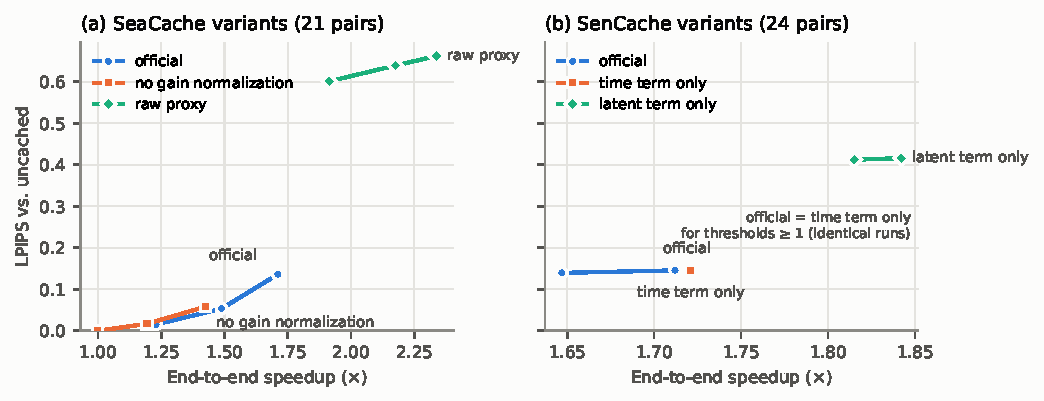
\includegraphics[width=\linewidth]{figures/ablation.pdf}
\caption{Ablations: each variant against the official policy on the same pairs.}
\label{fig:ablation}
\end{figure}
\textbf{SeaCache.} Replacing the SEA filter by the identity (raw proxy) makes feature differences look small, so the policy
reuses aggressively (refresh 0.10--0.25, up to 2.34$\times$) but LPIPS jumps to 0.60--0.66 and PSNR to 14\,dB---the videos
diverge from the uncached output. Removing gain normalisation has the opposite effect: scores grow, reuse falls (no reuse at
all at 0.1, PSNR $=\infty$) and the variant traces a curve slightly behind the official one (e.g.\ LPIPS 0.058 at 1.43$\times$
vs.\ 0.053 at 1.49$\times$). The filter is therefore what makes the proxy track perceptually relevant change; normalisation
mainly rescales the threshold.

\textbf{SenCache.} With the latent term only, the policy skips more (refresh 0.28) and LPIPS rises to 0.41; with the time
term only, results are identical to the official policy for thresholds $\geq1$ and differ only at 0.5 (LPIPS 0.146 vs.\
0.139). The time term thus governs SenCache's decisions on this configuration, while the latent term acts as a mild safety
margin at the smallest threshold. The calibration-size ablation from the plan was not run.

\subsection{Held-out test with frozen thresholds}
\pending{} Paired fidelity (3{,}000 cached vs.\ 750 uncached test videos) and VBench dimensions on the 110-prompt subset,
with the same bootstrap procedure, will be inserted here when the frozen test completes.

\subsection{Qualitative and failure-case analysis}
\pending{} Synchronised frames from one independently selected success case and one failure case (highest LPIPS) per
method at the frozen settings.

\section{Discussion and Limitations}
\textbf{Hardware changes the budget.} The same policies give 2.4--2.9$\times$ denoising speedup but only 1.5--1.7$\times$
end-to-end on A100 because the FP32 VAE decode is a large fixed cost. Reported end-to-end speedups therefore depend on the
GPU and on the decoder, and budgets should be stated for the part that caching accelerates.

\textbf{Calibrated vs.\ adaptive signals.} MagCache's static, calibrated schedule beats TeaCache's timestep proxy at equal
cost, and SeaCache's content-adaptive proxy is best at low and moderate budgets. Adaptivity is valuable only when the proxy
tracks perceptual change, as the raw-proxy ablation demonstrates.

\textbf{Limitations.} One backbone (1.3B), one resolution and sampler; calibration profiles were reused rather than
re-measured (their cost is not reported); validation used 29 common prompts (86 pairs) because cells completed on another
GPU were excluded; ablation timings come from a warm single-repeat protocol; agreement metrics measure deviation from the
uncached video, not quality; the VBench evaluation uses a custom 110-prompt subset.

\section{Conclusion}
On Wan2.1-T2V-1.3B, residual caching gives 1.5--1.7$\times$ end-to-end (2.1--2.9$\times$ denoising) speedup on A100. At
matched cost MagCache is markedly more faithful than TeaCache, SeaCache is the most faithful policy at low and moderate
budgets and the only one with content-dependent schedules, and its spectral filter is the component that makes this work.
SenCache's behaviour is dominated by its time term. \pending{} [held-out test conclusion].

\section*{Team Contributions}
\begin{tabularx}{\linewidth}{@{}p{0.26\linewidth}YY@{}}\toprule
Member & Contribution & Cross-check / evidence\\\midrule
\fillin{name} & \fillin{completed work} & \fillin{review or run record}\\
\fillin{name} & \fillin{completed work} & \fillin{review or run record}\\\bottomrule
\end{tabularx}

\section*{Reproducibility Statement}
\sloppy
Run directory \texttt{ce6190-runtime/a100x8-20261110}: \texttt{manifest.jsonl} (validation grid), \texttt{phaseD/} (ablation
manifest), \texttt{phaseC/} (test subset, frozen config, manifest); per-run \texttt{metrics.json}, \texttt{trace.json},
frames and MP4 in \texttt{results/}; acceptance reports in \texttt{acceptance/}; fidelity records in \texttt{eval/}; official
aggregation and the tables/figures of this report from \texttt{analysis/} (\texttt{make\_tables.py},
\texttt{make\_figures.py}); environment lock in \texttt{logs/pip-freeze.txt}; all decisions and deviations, with
timestamps, in \texttt{PLAN.md}.

\bibliographystyle{plainnat}
\bibliography{references}
\end{document}
